% interactapasample.tex
% v1.05 - August 2017

\documentclass[]{interact}

\usepackage{epstopdf}% To incorporate .eps illustrations using PDFLaTeX, etc.
\usepackage[caption=false]{subfig}% Support for small, `sub' figures and tables
%\usepackage[nolists,tablesfirst]{endfloat}% To `separate' figures and tables from text if required
%\usepackage[doublespacing]{setspace}% To produce a `double spaced' document if required
%\setlength\parindent{24pt}% To increase paragraph indentation when line spacing is doubled

\usepackage[longnamesfirst,sort]{natbib}% Citation support using natbib.sty
\bibpunct[, ]{(}{)}{;}{a}{,}{,}% Citation support using natbib.sty
\renewcommand\bibfont{\fontsize{10}{12}\selectfont}% To set the list of references in 10 point font using natbib.sty

%\usepackage[natbibapa,nodoi]{apacite}% Citation support using apacite.sty. Commands using natbib.sty MUST be deactivated first!
%\setlength\bibhang{12pt}% To set the indentation in the list of references using apacite.sty. Commands using natbib.sty MUST be deactivated first!
%\renewcommand\bibliographytypesize{\fontsize{10}{12}\selectfont}% To set the list of references in 10 point font using apacite.sty. Commands using natbib.sty MUST be deactivated first!

\theoremstyle{plain}% Theorem-like structures provided by amsthm.sty
\newtheorem{theorem}{Theorem}[section]
\newtheorem{lemma}[theorem]{Lemma}
\newtheorem{corollary}[theorem]{Corollary}
\newtheorem{proposition}[theorem]{Proposition}

\theoremstyle{definition}
\newtheorem{definition}[theorem]{Definition}
\newtheorem{example}[theorem]{Example}

\theoremstyle{remark}
\newtheorem{remark}{Remark}
\newtheorem{notation}{Notation}

\begin{document}

\articletype{Manuscript Submission to \emph{Building Research and Information} Journal}% Specify the article type or omit as appropriate

\title{Spacematch: AI-enhanced platform to improve spatial utilization and comfort at workplaces using occupant environmental preferences and IoT data}

\author{Tapeesh Sood\textsuperscript{a},
Patrick Janssen\textsuperscript{b},
and Clayton Miller\textsuperscript{a}$^{\ast}$\thanks{$^\ast$Corresponding author email: clayton@nus.edu.sg}\\
\vspace{6pt}
\textsuperscript{a}{\em Building and Urban Data Science (BUDS) Lab, Department of Building, School of Design and Environment (SDE), National University of Singapore (NUS)};\\
\textsuperscript{b}{\em Department of Architecture, School of Design and Environment (SDE), National University of Singapore (NUS)}
}

\maketitle

\begin{abstract}
%Modern commercial building management are embracing the concept of activity-based work spaces. This strategy improves the spatial efficiency of office work environments and reduces the cost per occupant. However, the impacts on the personal satisfaction of those occupants is not always positive. Occupants have lost a sense of desk ownership, more time is spent finding an optimal work space, and environmental comfort is often one-size fits all. The personal indoor environmental quality (IEQ) and wellness aspects of office work spaces are important to the productivity, health, and satisfaction of those occupants. This paper describes a new approach to enhancing activity-based work spaces that learns the environmental comfort preferences of occupants and matches them with a catalogue of available work spaces. This recommendation system empowers occupants to maximize their comfort and efficiency and enables operations staff to optimize the control of their comfort creation systems (HVAC, lighting, etc.) by grouping occupants with similar preferences. This approach is illustrated through a pilot implementation on a university campus using a smart phone application.


Workplace operators face enormous pressure to drive down rental costs by maximizing spatial utilization. But, as operators aspire to grow headcount within existing footprint, it often results in taking away what makes occupants comfortable and productive in exchange for cost savings. One way to tackle this is to increase the frequency and volume of occupant feedback in buildings. However, identifying occupants preferences frequently using traditional human feedback collection methods such as surveys, interviews presents significant challenges of scalability among other limitations. This paper showcases 'Spacematch' - a web based platform for easy collection of real-time personal environmental comfort preferences in flexible workspaces to improve environmental comfort and spatial utilization. This new approach connects occupants with a catalog of available work desks using a mobile application, enables them to easily provide environmental feedback in real-time, and facilitates merging this feedback data with indoor environmental values, from fixed room sensors, to optimize space and energy use by grouping occupants with similar preferences. The study covers a pilot implementation of the preliminary version of the platform with 25 research participants over a month at a university campus - and shares the challenges faced during implementation and next steps in its advanced development.

\end{abstract}

\begin{keywords}
Co-working; Personal environmental comfort; Spatial efficiency; Recommendation systems; Activity-based work spaces
\end{keywords}




\section{Introduction}
%Workplaces today face challenges as operators look to offset high rental costs by growing occupant headcount within their existing footprint. Equally, rapid changes in technology and nature of work in the the past few years have led them to rethink spatial density and utilization.  

In the past few years, rising corporate real estate (CRE) costs, rapid changes in technology and nature of work have rendered traditional modes of working---where occupants are designated one work desk each for long periods---inefficient. Today, 37\% of all office spaces are empty on any given workday \citep{jll} - which equates to approximately 150 billion dollars annually in unused space globally \citep{cbre}. These challenges are pushing building operators to rethink occupant density and spatial utilization in workplaces.  


In a recent survey, while 95\% of CRE professionals believed that workplaces influence occupant productivity and comfort, only one third measured that impact. Most others solely considered traditional cost based measures and metrics to quantify workplace density and utilization \citep{gensler}. Based on past studies, heavy reliance on cost based measures generally results in operators taking away amenities that make occupants comfortable and productive in work environments for cost savings - like replacement of cubicles with benches to accommodate a larger headcount, removal of informal collaboration spaces for more desks or taking away of employee storage space all together \citep{cbre}.

%One of the reasons for this situation is the heavy reliance of operators on traditional cost based measures and metrics to quantify workplace density and utilization - such as cost per square feet dedicated to a workstation or an occupant 
 

In response to these challenges, new and dynamic ways of working are evolving rapidly . These approaches aspire to simultaneously balance operator's---cost and space saving---demands with flexibility and comfort needs of employees through enabling occupant mobility. Through most the occupant is able to work flexibly by choosing different places within the workplace rather than being assigned a fixed desk as the one primary place of work. Once occupants are dynamic in the ways they use space, its easier to recapture underutilized spaces by operators \citep{cbre}.

%When executed well, this improves the real estate bottom line whilst enhancing overall occupant comfort, choice and control in workplaces

Workplace strategies of this kind are referred in various ways by industry stakeholders, with frequently used references such as hot-desking, co-working, desk sharing, flexible working, activity based working, office hoteling and so on. Though each strategy varies slightly from the other, most promise benefits of improved spatial utilization and cost savings for operators while increasing overall comfort, choice and control for occupants \citep{Engelen2018IsReview}. Understandably, an increase in adoption of these concepts can be seen in the growing co-working industry by companies such as WeWork\textsuperscript{\textregistered} and Regus\textsuperscript{\textregistered} across the globe.  %Equally, a large recent survey of spaces utilizing one such strategy showed that the main motivations for occupants to work in such a workplace is because it allowed access to an inspiring work environment \citep{Weijs-Perree2018AnalysingCharacteristics}.

However, limitations of such approaches have also been documented. A study focused on a sociological analysis of one approach showed a loss of everyday work space ownership giving rise to practical and social tensions within the organization \cite{Hirst2011SettlersHot-desking}. And, another study found lower than expected satisfaction with activity based working environments due to rare switching of different activity settings \citep{Hoendervanger2016FlexibilityEnvironments}. 

%However, limitations of such approaches have also been documented by past studies. A study focused on a sociological analysis of one approach showed a ``loss of everyday work space ownership giving rise to practical and social tensions and shifts hot-deskers’ identification with the organization \cite{Hirst2011SettlersHot-desking}.`` Another study found lower than expected satisfaction with activity based working environments due to many works rarely switching between different activity settings \citep{Hoendervanger2016FlexibilityEnvironments}. 

As organizations evolve, they are rightfully nervous of ill-conceived applications of new strategies to their workplaces - which may disrupt business and culture purely for the sake of cost savings. They seek---easy to use, scalable---solutions which provide actionable insights that help justify space and cost savings without sacrificing occupant comfort and performance in workplaces. 

%Implementing these new ways of working will not drive down the cost per seat. Instead, they aim to drive down the cost per person by optimising the utilisation of the space, which CBRE refers to as “dynamic density”. This allows staff to work flexibly through choosing different places to work within the office rather than being assigned a fixed desk as the one primary place of work. Once workers are dynamic in the way that they use space, then it becomes quite straightforward to recapture latent underutilised space or what is generally referred to as desk sharing. 


%Activity-based working (ABW) is a major movement in commercial buildings. In these strategy, occupants have no permanent workstation; instead, they are given a range of space choices based on their activity and immediate needs. This space planning strategy, also known a \emph{hot desk} strategy, is becoming more common as a means of increasing the space use utilization of offices. An extensive literature review found that ABW results in an increase of interaction, communication, and control of time \. However, the same study found that these spaces can results in reductions of occupant concentration and privacy. ABW is a common strategy in the growing industry of co-working spaces by companies such as WeWork\textsuperscript{\textregistered}. 

  
%These challenges motivate the development of techniques that solidify the space and social advantages ABW while increasing the probability that an occupant will find and use the right space for them at the right time.





\subsection{Understanding indoor environmental comfort in buildings}
%In addition to space use allocation, indoor environmental comfort is at the forefront of building performance analysis.
Occupant dissatisfaction with indoor environments has far reaching economic implications for workplaces. Various sources estimate that 80-90\% of the costs of a building are associated with workers salaries, compared with only 3\% being associated with owning and maintaining the property \citep{Creativeandproductiveworkplaces, kats2003green, wilson2005making}. As people typically spend over 90\% of their time indoors, the quality of the indoor environment influences their comfort, performance, health and wellbeing. Occupant dissatisfaction with indoor environments can result in health impacts, absenteeism, and poor productivity \citep{MiltonDonaldK.P.MarkGlencross2000}. As an example of health-related issues, a comparison of 12 field studies from United States and six other countries in Europe, covering a total of 467 buildings with 24,000 occupants, the air-conditioned buildings (with or without humidification) showed between 30\% and 200\% more cases of sick building syndrome symptoms than in the naturally ventilated buildings' occupants \citep{Evolvingopportunities, ventilationsystemtype}. A recent survey in 2012 of 52,980 occupants in 351 office buildings found that 50\% of the occupants were dissatisfied with their indoor environment \citep{Frontczak2012QuantitativeDesign}. 

% The over-conditioning and over-sizing of comfort control systems also has an impact on energy, and therefore the carbon emissions of buildings as well.

In response to these challenges, research in indoor occupant comfort has accelerated over the last twenty years. One of the many paradigm shifts has been the movement away from traditional, physically-based deterministic models - an analysis of the predicted mean vote (PMV) and predicted percentage of dissatisfied (PPD), the two most widely used comfort indices, showed that their accuracy is only 34\% across dozens of comfort studies in the last few decades \cite{CHEUNG2019205,FOLDVARYLICINA2018502}.
 
Recent research efforts have progressed towards adaptive comfort models \citep{Ferrari2012AdaptiveIndices, Nicol2013AdaptiveWorld, vanHoof2010ThermalPractice}, which rely heavily on human behavior. According to these models, discomforting changes in thermal environment are followed by behavioral change in people to restore comfort. Such actions could include reducing individual activity levels or even opening a window. The main effect of such models is to increase the range of conditions that designers can consider comfortable, for instance, naturally ventilated buildings in the tropics where occupants have a greater degree of control over their thermal environment.

Despite these advancements, even adaptive comfort models follow a one-size-fits-all approach that ignores the personal aspect of comfort; this is like expecting everyone to have the similar preferences for food, music, or style; all subjective attributes of a person’s personality. Further work on adaptive models is needed to identify comfort preferences on an individual basis and not only based on the thermal conditions.  

Recent studies have shown that individual differences in comfort preferences and personality could explain variations in environmental perception between occupants exposed to the same conditions \cite{cheung2019analysis, livcina2018development}. One way researchers have addressed this is through personal comfort models which predict individual thermal comfort responses rather than the average response of a larger population i.e an entire floor or a building \cite{kim2018personal}. These models generally leverage  machine learning techniques and the Internet of Things (IoT) technologies to evaluate individual thermal comfort requirements based on data collected in everyday conditions. This approach has demonstrated very high prediction accuracy well beyond that of the traditional models \cite{kim2018personal1}.

%\begin{figure}
%\centering
%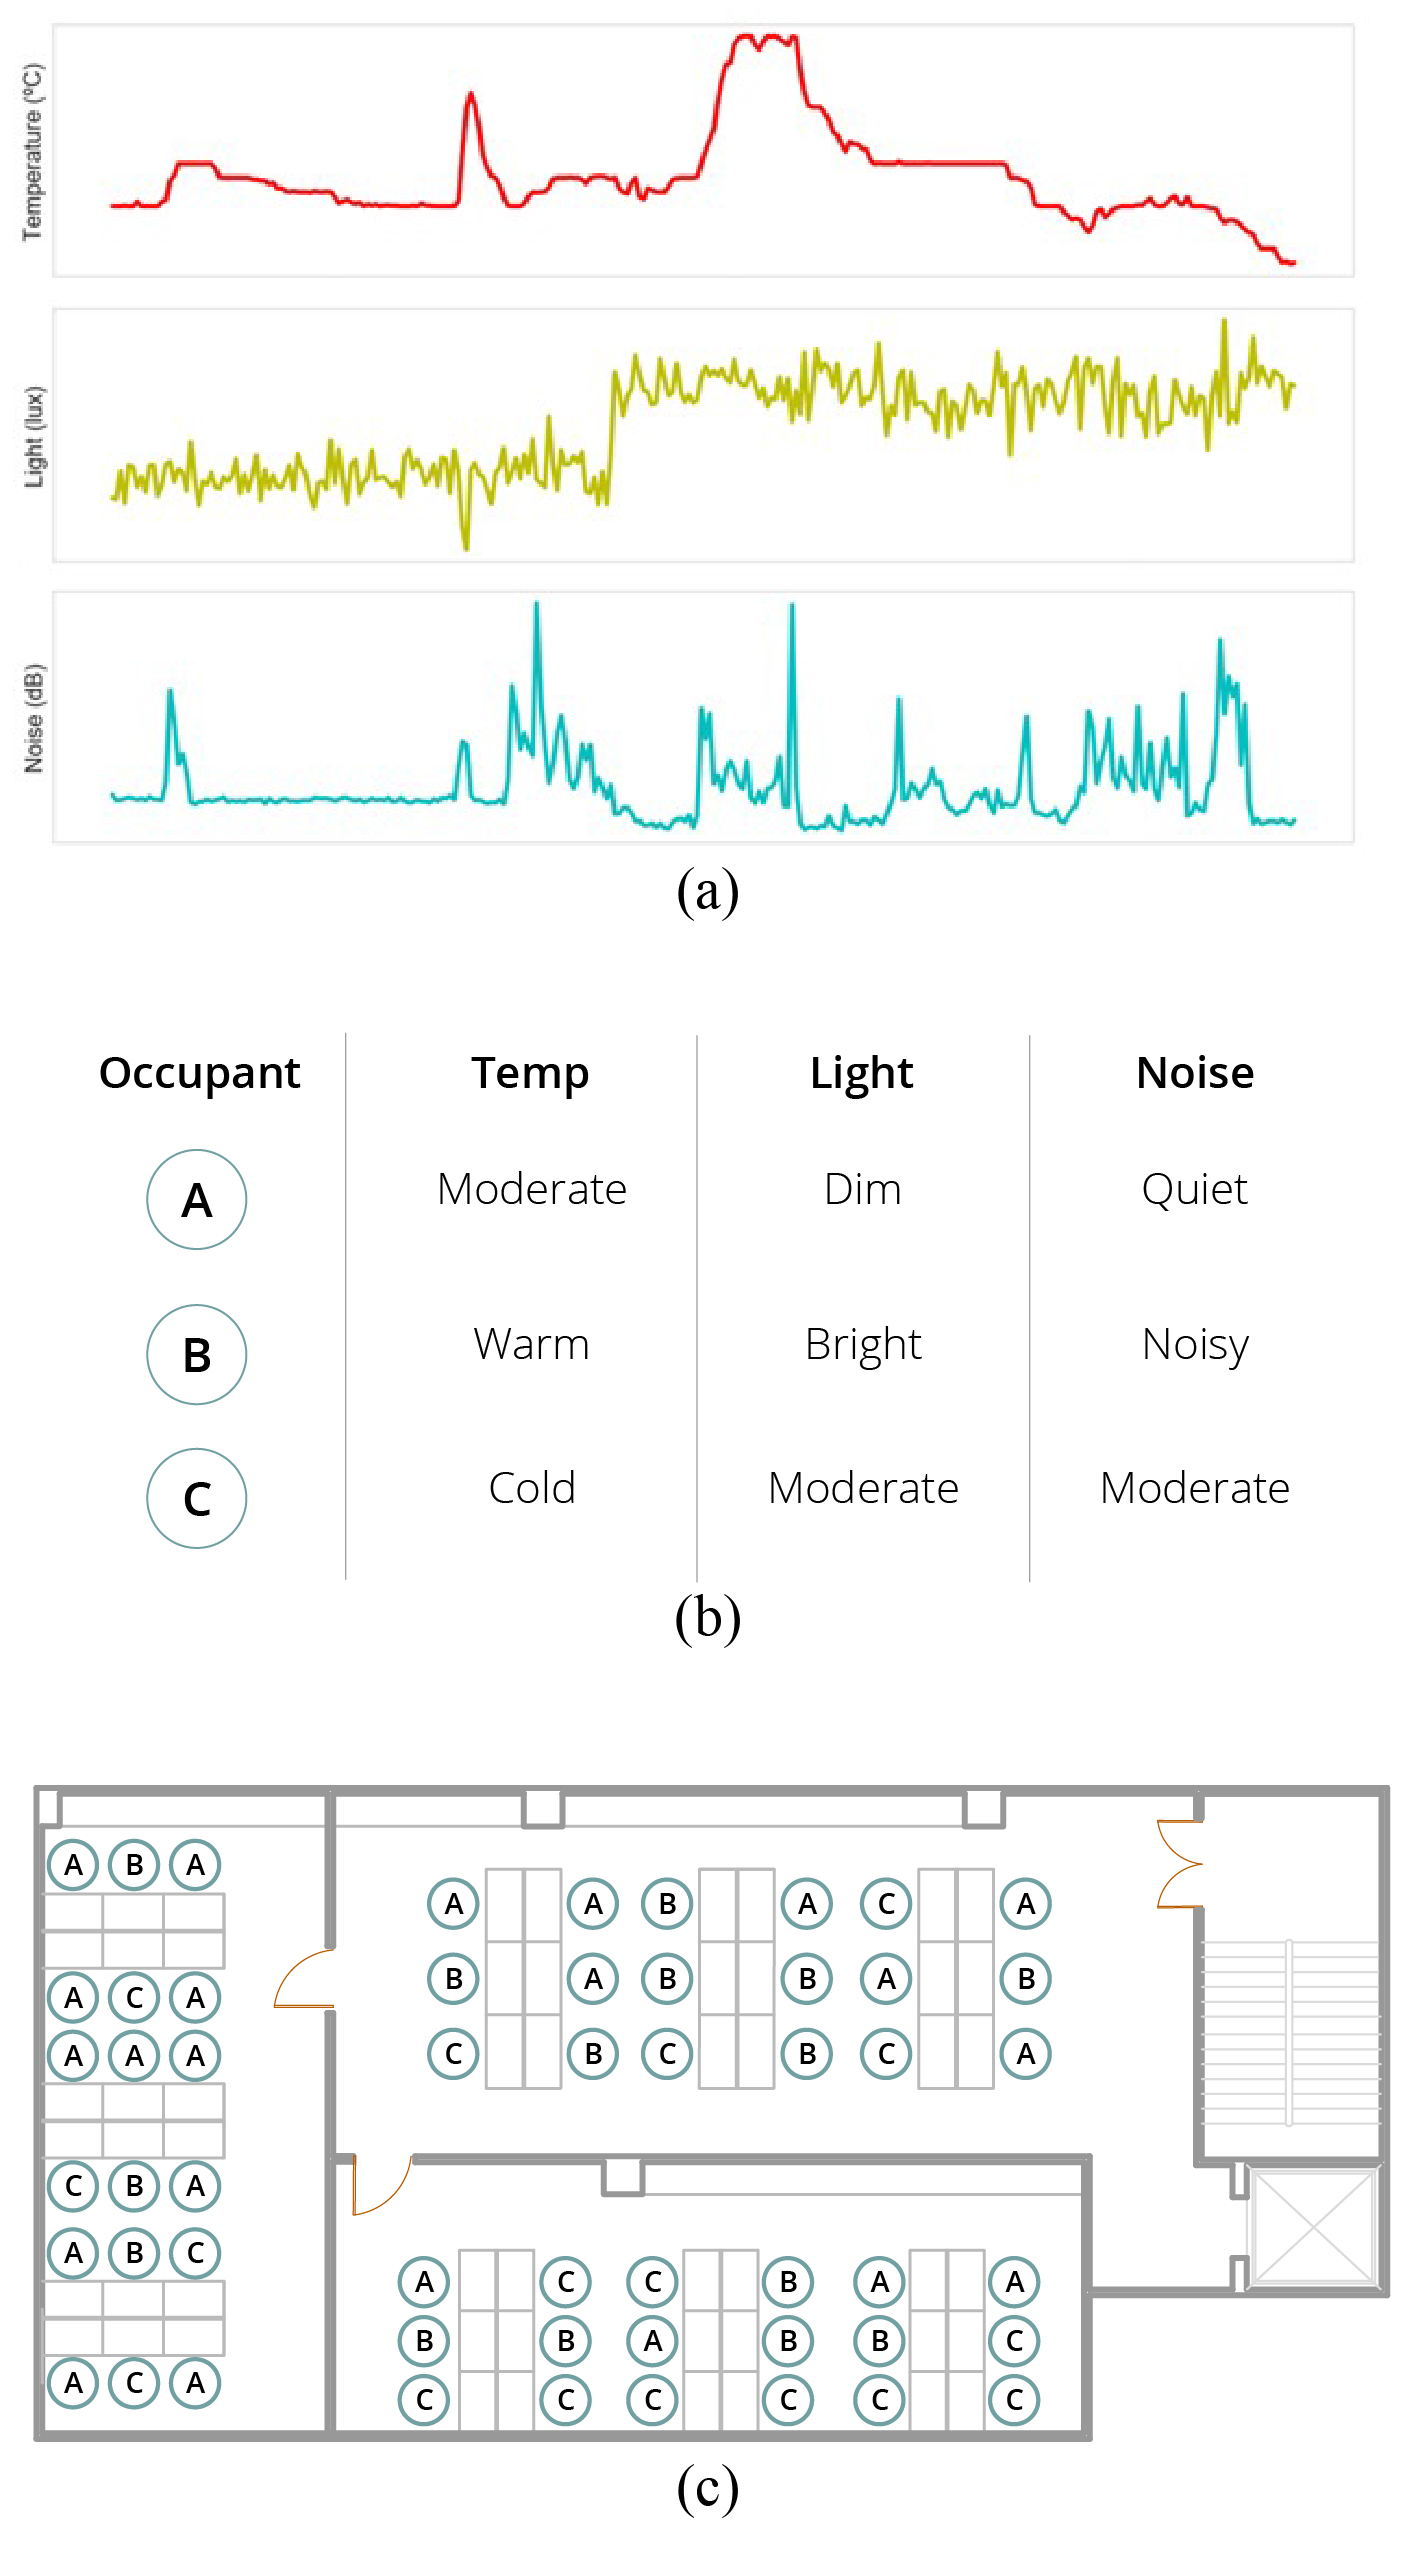
\includegraphics[scale=0.8]{figures/Fig1a.jpg}
%\caption{Conventional IoT environmental quality data} \label{iot-example}
%\end{figure}




\subsection{Building systems’ response to indoor environmental challenges}
In addition to the work in comfort models, a large amount of research has also been done to improve the systems that respond to comfort needs. Various mechanical systems technologies such as radiant systems and decentralized and personalized ventilation attempt to address comfort problems. These contemporary innovations focus on the ability of a building to adapt to its occupants by tracking them and modifying each person's immediate personal climate to meet their individual needs \citep{Brager2015EvolvingComfort}. 

Personalized control system approaches are problematic as the spatial resolution of most existing climate, lighting and noise control technologies is not great enough in flexibility and responsiveness to make this approach feasible. Even more innovative, decentralized and personalized comfort systems are unable to create the response and resolution needed to create individualized comfort zones in a practical way. Additionally, smaller and more decentralized systems create more maintenance tasks and complexity within the building systems \citep{VESELY2017223}.

To meet these challenges of decentralization, a balance needs to occur between personalizing spaces and maintaining the economies of scale that centralized systems provide. Creating small zones of personal comfort for all occupants should be used sparingly in very specific space use types, while most other spaces can be conditioned to meet the needs of a subgroup of people. 




\subsection{Collecting human comfort feedback in buildings}
Today, researchers and building owners install a wide range of IoT devices that measure various environmental conditions such as light, noise, and particulates levels, in addition to the conventional temperature and humidity metrics. 
%Figure~\ref{iot-example} illustrates several examples of environmental sensor data from a building.
Although IoT sensors have become low cost and ubiquitous, the data from these devices are often not utilized to their full potential. Comfort models, even adaptive ones, only set thresholds to which these sensor data points can be compared. The key element in putting these data in context is subjective and physiological feedback from people who inhabit the environment. Collecting this type of data would empower more specialized and nuanced comfort models to be developed in a scalable way \cite{ltpaper}.

But, what may suit one group of occupants may be unacceptable for others. Even though its understood that differences in individual comfort preferences exist \cite{WANG2018181}, their quantitative identification presents significant challenges in field conditions for researchers and practitioners.

One way to tackle this situation is to increase the frequency and volume of building occupant user feedback. The contemporary methods of human feedback collection include structured surveys or interviews - on-line or off-line, in person or remote. However, such conventional approaches have a number of shortcomings \cite{oecd}. One major drawback of these methods is the lack of scalability - it’s difficult to collect large sample data sets due to the administrative, financial and other operational overheads associated with these approaches. Furthermore, other factors such as lack of knowledge (respondents do not know the answer to a question, but answer it anyway), lack of motivation (respondents may not process questions fully) and failures in communication (survey questions may be unclear or misunderstood) result in an increased risk of biases and respondent heuristics in traditional survey responses \cite{bradburn2004asking}.

As sensor adaptation in built environments continues to grow, new technologies and modern data capabilities equip researchers and practitioners to capture dynamic human feedback effectively. But this approach presents significant challenges in collection, analysis, processing and visualization of large data sets from building occupants. There is a need of easy to use, scalable solutions that help identify and quantify occupant comfort preferences for operators to make workplaces more comfortable and productive.


\subsection{Improving flexible workspaces by using personalized environmental comfort preferences of occupants and IoT data}
%Adaptive comfort has long been a vision of the building industry from the perspective of the occupants \emph{tolerating} the potentially sub-optimal conditions that a comfort control system provides \citep{Nicol2013AdaptiveWorld}. This paper outlines a vision of the word \emph{adaptive} encompassing the ability for occupants to make an informed decision about where they spend time. A previous study has use occupancy data to attempt to optimize the allocation of hot desk spaces using simulation and occupancy sensors \citep{Cooper2017AnData}.

This study addresses each of the previously mentioned challenges: easily collecting larger volumes of personalized data useful to occupants and operators, reducing the need for complex and problematic personalized comfort systems, and impacting flexible work spaces by improving spatial utilization and occupant comfort. 

This paper presents SpaceMatch - a scalable and easy to use platform for collection of personal environmental comfort preferences in flexible workspaces. This new approach connects occupants with a catalog of available work desks using a web based mobile application. The occupants can choose to use the work desk right away or reserve for later use. During use, the mobile application enables occupants to easily provide environmental comfort feedback for temperature, noise and light variables. 
For flexible workspace operators, it facilitates merging personalized environmental comfort data with other data streams---such as indoor environmental quality, occupancy and energy use data among others---to optimize space, energy usage and occupant comfort by grouping users with similar preferences. The study shares the development of the platform's fundamental features and also a pilot implementation of its preliminary version with 25 research participants over a month at the School of Design & Environment (SDE) at the National University of Singapore. 


%In this paper, we give an overview of the development of the concept of Spacematch: an artificial intelligence-driven (AI) spatial comfort suggestion system that will guide occupants to zones that match their environmental comfort preferences. These zones will be controlled according to the needs of a certain type of environmental preference personality, or clusters of people with similar needs. These comfort personality types will be created through an extensive set of experiments using environmental Internet-of-Things (IoT) sensor nodes combined with user feedback from an innovative space-booking smart phone application. This app will give occupants the ability to find and reserve spaces. In addition, the plug loads for the user would be turned on automatically upon starting their work session by scanning a QR code. Their power consumption would be monitored and reported throughout their time at the desk. Through this useful booking process, occupants will also be given a chance to leave a star rating of their thermal, visual and aural comfort experience within their individual space. This rating can be combined with an array of IoT sensor data sources. These type of sensors measure indoor temperature, humidity, various gases, noise, lighting, and presence levels. An individual’s star rating history will begin to develop a profile of their comfort preferences as combined with the measured data from their environment. The data from numerous study participants will be clustered to create the phenotypes of comfort that could be grouped into the same areas. Once the model recognizes what type of comfort personality a person has, the artificial intelligence model will then be used to predict what spaces best match that individual and are available to be used in the time-frame desired. This type of trained classification model is the similar to the algorithms that organizations like Amazon\textsuperscript{\textregistered} use to match products to potential consumers based on their history. To the authors' knowledge, this is the first study to use a recommendation system driven by sensor data and thermal comfort feedback to power an ABW strategy.



%\section{Methodology}
%The hypothesis of this recommendation system is to test whether certain groups of occupants can be segmented according to their comfort preferences and whether this segmentation is realistic in the context of an actual building case study. This platform is designed test whether suggesting spaces that match a person’s previous preferences has an impact on their satisfaction as compared to a baseline level of satisfaction for an activity-based scenario. We also want to test whether people’s comfort perceptions match the physiological data from the environmental data from the IoT sensors. This approach is significant as it creates an unprecedented amount of data that can quantify thermal comfort personality that tests a new method of designing and allocating space in buildings. 


%In this section, we describe a simplified scenario that illustrates the concept of a spatial recommendation system. Imagine a scenario in which people can assign a feedback rating to a space based on their thermal, aural, and visual comfort. People would use a smart phone app to reserve a space and then leave comfort feedback in the form of a five-star rating when they finish using the space. This simple feedback on a useful process is similar to the methods that commonly-used apps like Uber and Airbnb utilize. These star ratings are used to annotate collected data from IoT. Figure~\ref{iot-example-annotated} illustrates the same time range as Figure~\ref{iot-example}, however the time range is segmented into zones of utilization. These zones are given specific ratings by three theoretical people: Persons A, B, and C. These three people respond to the conditions in each zone in different ways. Their preferences are recorded through this process, providing a way to develop a personality type for each of them. Person A enjoys a dim, quiet, and moderately conditioned space, while Person B is into a more active environment with a bit of noise and brightness. Person C likes a cooler environment that is not dead silent. As the person updates their star ratings, their preferences are used to build a recommendation engine that can predict what space will best meet the needs of the person.

%With these three theoretical personalities, we can further develop this scenario in the context of an activity-based workstations. Figure~\ref{space-plans} illustrates the status quo for these types of layouts. People basically sit down in various spots throughout the floor plan. Sometimes aware of their comfort needs, but often just sitting anywhere there’s an open spot. To create so many individual personal comfort zones would require dozens of individual systems and the person’s control and preferences would need to be collected somehow. We hypothesize that a recommendation engine trained with people’s preferences would be able to group people with the same personality type as seen in Figure~\ref{space-plans}. These people are given information that guides them to spots that are more likely to satisfy them. In this case, there are only three major comfort zones, thus the mechanical, lighting and envelope systems can respond with less complexity and less equipment. And the occupants will also achieve a higher level of satisfaction on average.

%\begin{table}[]
%\centering
%\begin{tabular}{lllll}
%Example Personality & A & B & C \\
%\hline
%Temperature & Pleasant & Warm & Cold \\
%Noise & Quiet & Noisy & Moderate \\
%Lighting & Dim & Bright & Ambient
%\end{tabular}
%\caption{Example indoor environmental quality personalities}
%\label{personality-types}
%\end{table}

\section{Methodology}
A pilot study was designed to test SpaceMatch in field conditions with 25 research participants at SDE. A total of 1182 environmental feedback points were collected over a month. A total of 36 desks in six different zones, split between two buildings, were identified as shown in Figure \ref{fig:pilot}. Differences in average temperature, light, noise levels, desks availability and zone accessibility were important considerations in selecting each zone for the experiment. Desks in each zone were arranged in proximity of fixed sensors measuring seven attributes in real-time: temperature, humidity, noise, light, carbon-dioxide, volatile organic compounds and presence. Every zone offered flexible work desks--research participants weren't assigned any desks---but there arrangement differed slightly. In some zones, desks were arranged to promote collaboration - the desks were aligned such that participants could face each other while working. In others, the arrangement enabled solitary, personal work. Each desk was identified through a unique label containing the desk number, room name and a QR code for connecting the desk to the progressive web application as shown in Figure \ref{fig:framework}.

Each participant in the experiment used the interactive mobile application to reserve and use work desks as shown in Figure \ref{fig:app}. Users could search for available work desks within two buildings at SDE. Once they chose the building, users could progress to select the room and desk to use. Users were provided with more information about the room and real-time indoor environmental quality through the ``Info`` and ``Dashboard`` features of the application as shown in Figure \ref{fig:app}b. 

The application provided options between using the desk right now or reserving it for later. To start using a desk, users had to scan the desk's QR code label using an inbuilt QR code scanner in the application. A minimum two hour time slot for a work session was provided for each desk booking. Users could also choose to extend their work sessions in two hour multiples as per their requirements using the application. During use, the application prompted users to provide environmental feedback for temperature, light and noise levels through a 3-point scale as shown in Figure \ref{fig:app}d. Prompts were configured such that they nudge users to provide feedback at the start, finish and once every half an hour of a typical two hour work session. 

The data from the users and fixed sensors was aggregated using a cloud-based, time-series database - which served as a platform for data acquisition, storage and error detection as shown in Figure \ref{fig:framework}. The combination of location-based user comfort feedback and fixed environmental sensor data allowed clustering analysis for personalized comfort profiles of users. These two data sources were merged through matching feedback location (spatially localized through desk QR code label), time of feedback collection (timestamp) and user ID (through an in-built anonymous authentication method).     



\begin{figure}
\centering
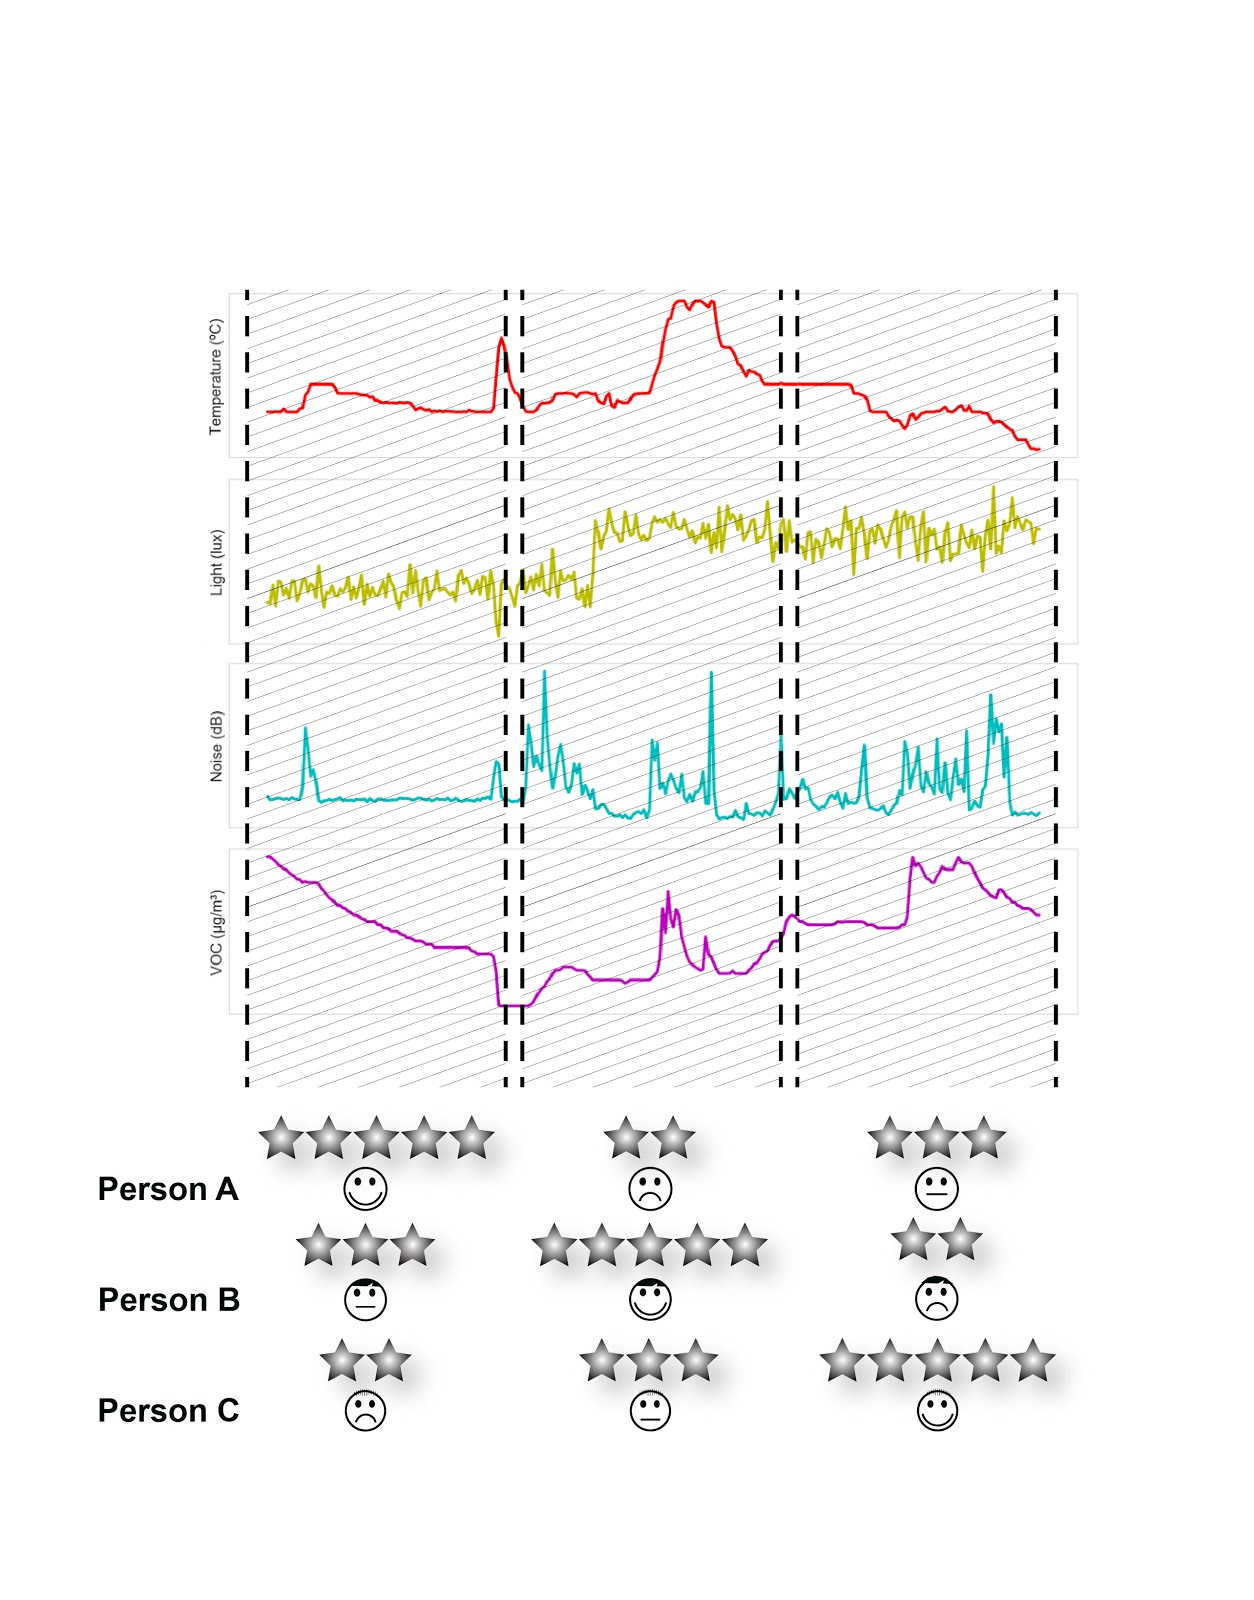
\includegraphics[scale=0.3]{figures/ieq_iot_annotated.jpg}
\caption{Pilot implementation setup} 
\label{pilot}
\end{figure}

\begin{figure}
\centering
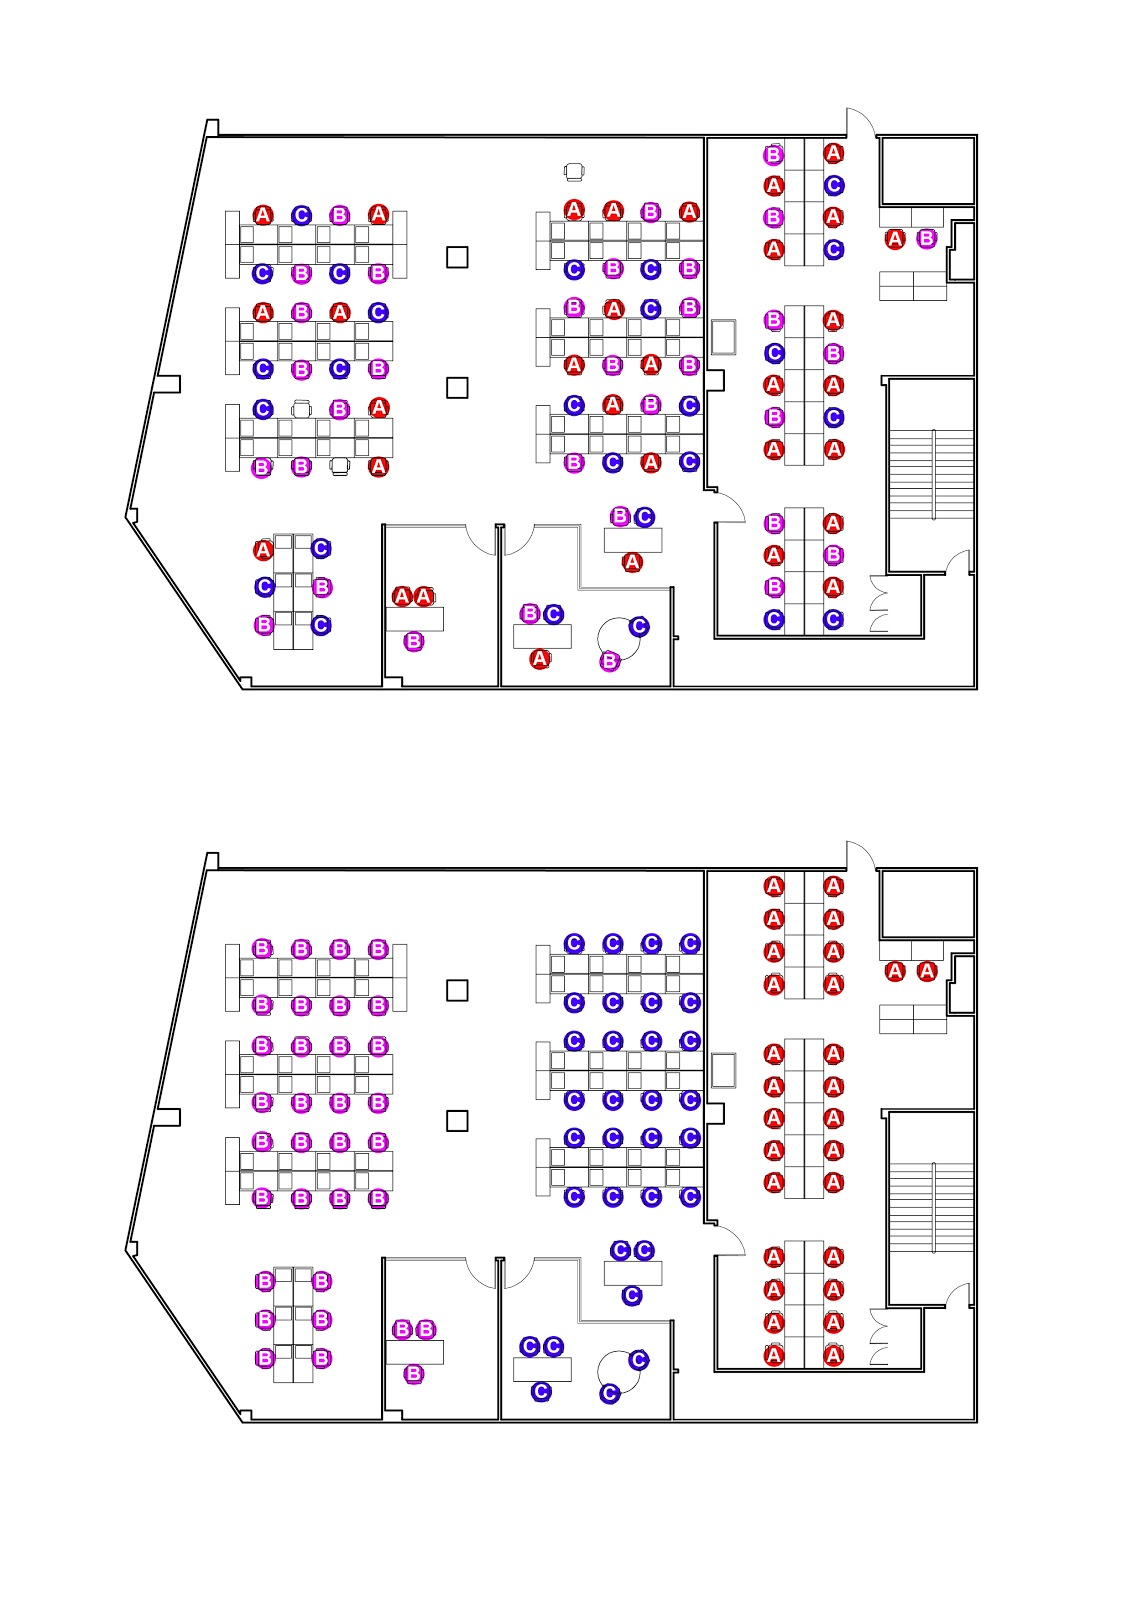
\includegraphics[scale=0.3]{figures/conventional_vs_recommedation.jpg}
\caption{components} 
\label{components}
\end{figure}

\begin{figure}
\centering
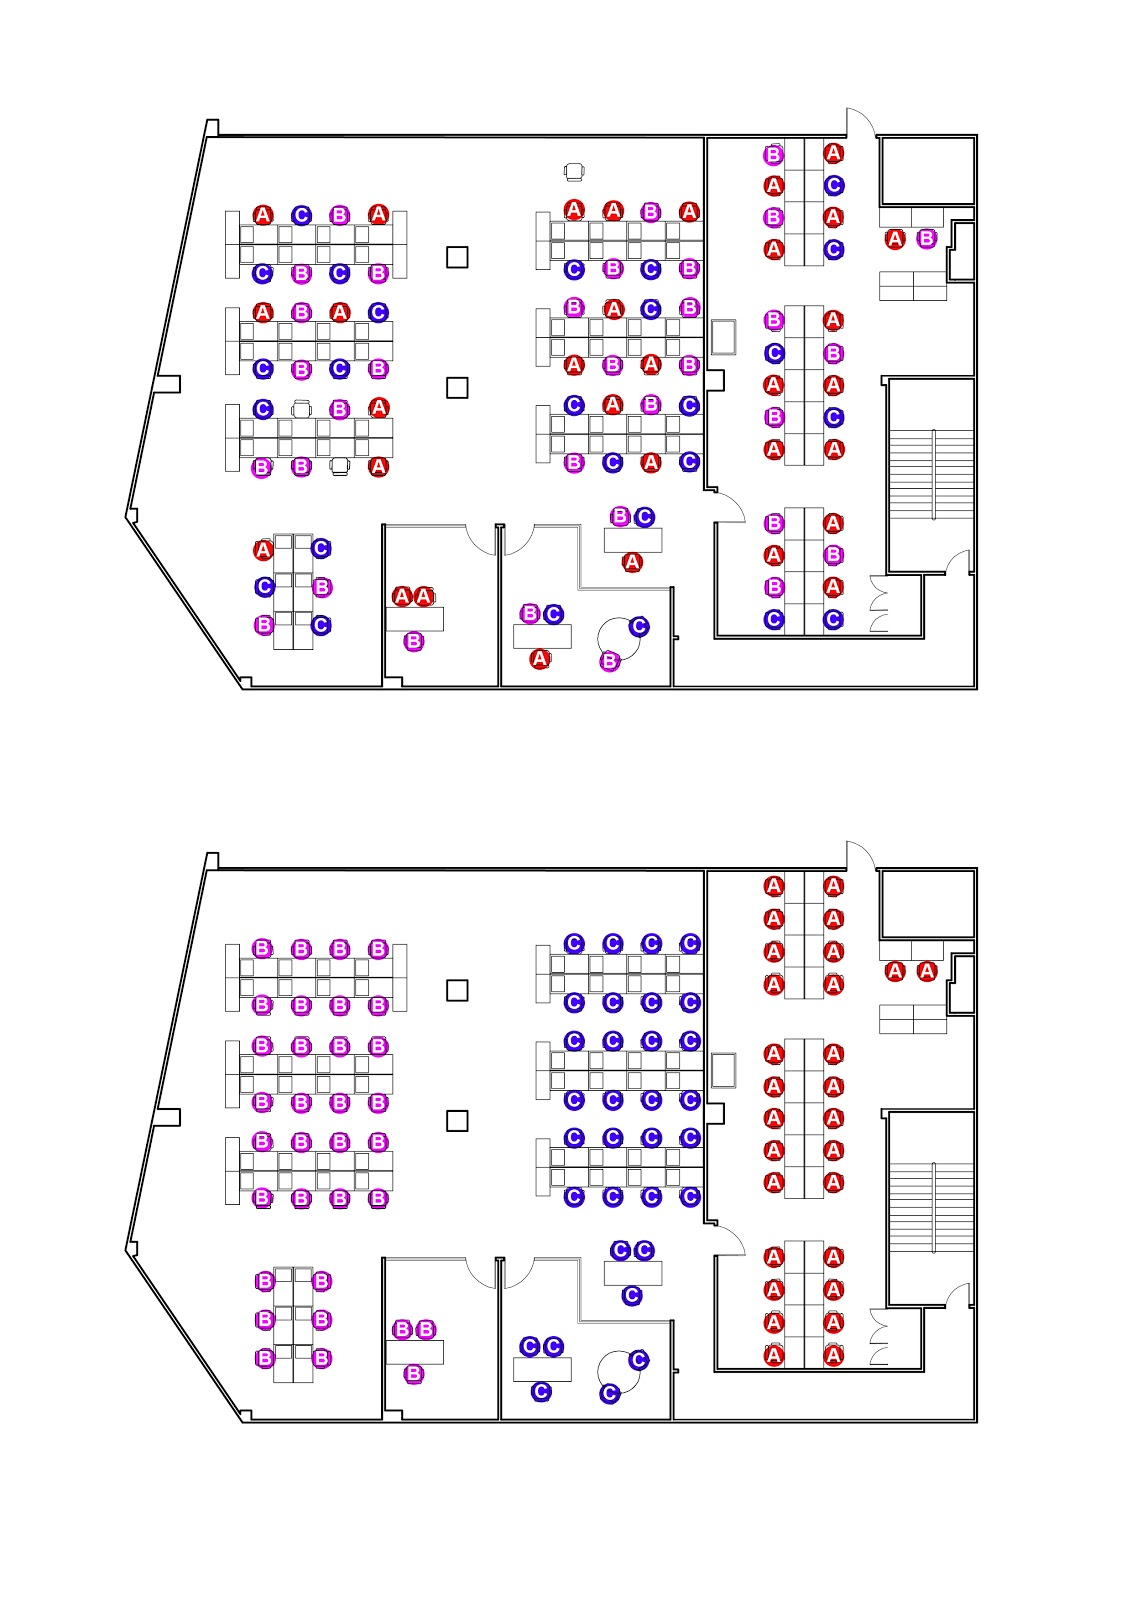
\includegraphics[scale=0.3]{figures/conventional_vs_recommedation.jpg}
\caption{The application framework} 
\label{framework}
\end{figure}

\begin{figure}
\centering
\includegraphics[scale=0.07]{figures/app.jpg}
\caption{The application} 
\label{app}
\end{figure}


%\subsection{Case study and participant overview}

%Various test case areas were be identified across campus that are applicable to the booking nature of the application. This includes the hot-desking spaces allocated for the SDE renovations as well area that are often utilized temporarily by staff, students or visitors. The deployment of a QR code sticker will occur at these locations and various signage advertising the application as a useful means of securing a place to work from afar will be explained. We will install Wifi-enabled Indoor Environmental Quality (IEQ) sensor nodes that will measure temperature, humidity, CO2, VOC, particulates, noise, light, and presence levels. 

%This set of experiments included XX individuals and they will be recruited from primarily amongst the staff and students of the School of Design and Environment (SDE), however all NUS students, staff and faculty were be considered. These participants will then utilize a developed smart phone application known as SpaceMatch to find and book spaces to set during the renovation of the SDE complex. SpaceMatch is a progressive web application, which means that it is technically a website, but has an appearance and functions similar to that of an ‘app’. SpaceMatch enables a user to scan a QR code located on the desk or on the wall of the space in order to make a booking, , leave feedback about thermal comfort, and learn more about the space in terms of sustainability features. Completing this task will also inform the participant’s location at that point in time. The participant will be aware that their location is recorded upon checking into the space. Upon completion of the use of a space, the participants would be asked to give feedback about the space using the questions seen in Figure 7. There will be three questions on a simplified three point scale. The first pane will ask if the participant is too hot, comfy, or too cold; the next question asks if the participant it is too quiet, comfy, or too noisy; and the last will ask if it is too dark, comfy, or too bright. The survey takes less than 30 seconds to complete as it is three simple feedback questions.

[%here insert screenshots of the latest spacematch demo version]

%This pilot field study was be conducted for xx weeks. Training  included a tutorial on how to use the application as well as details of the research study. This could occur in the days before the experiment begins or on the initial day. They are not required to utilize the desks on campus in any different way than their usual habits. They will be asked to simply utilize the application whenever they use a space in the test area in the SDE buildings. Some of the participants will carried a SENSg sensor device that measures temperature, pressure, sound, light, inertial measurement, step count, indoor/outdoor time, and travel pattern. Travel patterns is the approximate location of the subject based on Wifi triangulation. Participants will be informed in the consent process that the SENSg sensor will track their location. The participants will be asked to carry the SENSg devices with them during daytime hours, when they are on NUS campus at the very least, but are welcome to wear the device during the three month period. The SENSg device was designed and developed by researchers from the Singapore University of Technology and Design (SUTD) as a “Laboratory on a Lanyard” to enable Singapore’s National Science Experiment (https://nse.sg/sensg/about-sensg/). These 15 participants will also install a second smartphone application called FollowMee to be used for the 3 month period (installed on personal smartphones) (https://www.followmee.com/) that will track their location inside or outside the test case zone during daytime hours on weekdays from during the hours in which they are scheduled to be on the NUS campus or on their way to campus. This app uses the GPS of the participant’s smartphone for this tracking. 

%The participants can decide when the application starts and stops tracking by toggling the option in the application. They will be asked to set the start and stop times based on when they are on their way to campus or on their way home from campus. Participants’ location indoors while in the test zone will be based on the space that they utilize through their scanning of the QR code. Scanning the QR code supplements the GPS-based tracking of the participant that is done through the Followmee app. This app uses the GPS of the participant’s smart phone for this tracking. This supplementary data can inform where exactly within the building the participant is located - this is a knowledge that GPS often can’t provide. The location information and environmental quality feedback will be collected through their interaction with the space, will be coded with a unique, anonymized identifier. 

%Both of the smart phone applications (SpaceMatch and Followmee) did not collect any personally identifiable information. All personal information will be collected in person upon signing the consent form. Researchers might already have the name and email address of the test participants before signing the consent however these data would not be included in the personal data set until the consent form has been signed. The personal data set will be kept separate from the research data. The smart phone application will be coded to the personal information using an anonymous unique identifier token that cannot personally identify the test participants. The survey data collected through the smart phone applications was linked with the other data collected in the study through an anonymous token.

\subsection{Spatial implementation scenario and data collection}

QR codes were dispersed amongst the desks in the architecture department at the National University of Singapore.

[here show the test setup implementation in floor plans and photos of the QR codes]

\subsection{Thermal comfort personalities detected}

This will be about unexpected factors or new findings which were not accounted for initially in the experiment but influenced human comfort perception in co working environments

\subsection{Challenges and next steps}

This will be about the following:
\begin{itemize}
  \item Challenges experienced in field study implementation
  \item Challenges in collection of user feedback in intuitive ways
 \end{itemize}

\section{Conclusion}

Preliminary data shows X.

\begin{itemize}
	\item Segregation and clustering of users based on thermal comfort personalities
    \item Suggesting spaces that match an individuals previous preferences to have an impact on their satisfaction as compared to a baseline level satisfaction for a co working environment
    \item Design, allocation and management of spaces based on thermal comfort personalities in the future
\end{itemize}

\subsection{Future work}



\section*{Acknowledgement(s)}


\bibliographystyle{unsrtnat}
\bibliography{spacematch}

\end{document}

